%%%%%%%%%%%%%%%%%%%%%%%%%%%%%%%%%%%%%%%%%%%%%%%
% BEGIN STATISCH EVENWICHT
%%%%%%%%%%%%%%%%%%%%%%%%%%%%%%%%%%%%%%%%%%%%%%%
\chapter{Statisch evenwicht}

Dit college wordt afgesloten met een korte verhandeling over statisch evenwicht. Je zal leren
wat de voorwaarden zijn voor evenwicht en hoe daar mee valt te rekenen. Het hoofdstuk gaat
in zekere zin verder waar hoofdstuk~\ref{chap:newton} is gestopt. Je moet weer gedetailleerde
krachten analyses maken om problemen te doorgronden.
Stof uit Giancoli:
\begin{itemize}
\item Hoofdstuk 12.1 - 12.2
\end{itemize}

\section{Krachtmoment}

In deze paragraaf geven we een simpele definitie van het begrip krachtmoment, dat je
wellicht eerder hebt gezien tijdens VWO natuurkunde. 
 \begin{figure}[htbp]
\begin{center}
  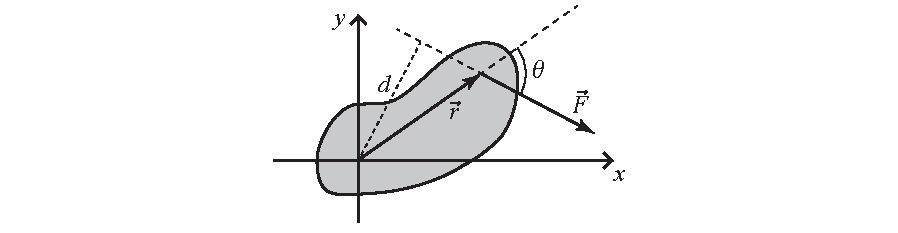
\epsfig{file=Krachtmoment.pdf, width=\textwidth}
\caption{{\it Variabelen benodigd voor de definitie van het krachtmoment.}}
\label{fig:torque}
\end{center}
\end{figure} 
Als je een object hebt zoals
bijvoorbeeld getekend in Fig.~\ref{fig:torque} waarop een kracht aangrijpt niet in het
zwaartepunt dan is het krachtmoment, $|\vec{\tau}|$ gedefinieerd als de 'kracht maal de 
arm', $d$, waarover deze kracht wordt uitgeoefend. Ofwel:
\begin{equation}
|\vec{\tau}| = |\vec{F}|\,d =|\vec{F}||\vec{r}|\sin\theta
\end{equation}
Let op dat hier expliciet over de grootte van het krachtmoment wordt gesproken. Wat in dit
college achterwege wordt gelaten is het vector-karakter van het krachtmoment. Al er een 
netto krachtmoment op een object wordt uitgeoefend kan een object gaan draaien om een 
bepaalde as. De dynamica van de draaibeweging echter, zoals die in hoofdstuk~11 van Giancoli
wordt besproken wordt voor dit college overgeslagen, maar komt in het $2^e$ jaar aan bod
tijdens het voortgezette klassieke mechanica college.  We gaan draaimomenten alleen
maar gebruiken voor onze studie van statisch evenwicht.                  

\section{Voorwaarden voor evenwicht}

Een goede vraag om mee te beginnen is, wat nou precies een statisch evenwicht is. In het 
kader van dit college verstaan we onder een  statische evenwicht een situatie waarbij een 
object in stilstand is, en dat ook blijft. Op zich klinkt een dergelijke situatie tranentrekkend saai, 
maar wat je in het algemeen leert van het onderzoeken van een evenwicht is wat voor krachten
er in en op een object worden uitgeoefend. Deze kennis is van levensbelang voor ingenieurs
die een brug of gebouw ontwerpen.

De eerste conditie waaraan een object moet voldoen, wil het in evenwicht zijn, is dat de som 
van alle krachten op dat object gelijk moet zijn aan nul:
\begin{equation}
\sum_i \vec{F}_i = \vec{0}
\end{equation}
Als dit niet het geval is dan gaat een object versnellen en is het dus niet in evenwicht.

Nu zou je misschien zeggen dat een object waarop de eerste conditie van toepassing is niet
gaat bewegen, maar dit is niet altijd het geval. De eerste conditie geeft enkel aan dat het 
zwaartepunt van een object niet van z'n plek komt, maar een object kan nog steeds gaan
draaien, als er een netto krachtmoment $\tau$ op het object werkt. Dus de tweede conditie
voor een statisch evenwicht is niet verrassend:
\begin{equation}
\sum_i \tau_i = 0
\end{equation}
De som van alle krachtmomenten om een bepaalde draaias moet gelijk nul zijn. Dit is alle
theorie die je nodig hebt voor het bestuderen van statische evenwichten. In het algemeen 
leveren beide evenwichtsvoorwaarden je een set van vergelijkingen op, waarmee je alle
krachten in een systeem kan bepalen. In de volgende paragraaf volgen een paar voorbeelden.

\section{Selectie van voorbeelden}

De voorbeelden 12-3, 12-5 en 12-6 uit Giancoli worden tijdens het college behandeld. 

\section{Wat moet ik weten en kunnen}

Je moet weten:
\begin{itemize}
\item Wat is krachtmoment.
\item Wat zijn de twee voorwaarden voor een statisch evenwicht.
\end{itemize}
Je moet kunnen:
\begin{itemize}
\item Analyseren hoe een evenwicht werkt.
\item Uitrekenen hoe groot de krachten zijn in eenvoudige problemen.
\end{itemize}

\section{Opgaven}

\begin{enumerate}
\item Giancoli hoofdstuk~12: 1, 11, 18, 22, 27, 32, 59, 62, 68, 70, 84, 85, 93, 95.
\end{enumerate}

%%%%%%%%%%%%%%%%%%%%%%%%%%%%%%%%%%%%%%%%%%%%%%%
% EINDE STATISCH EVENWICHT
%%%%%%%%%%%%%%%%%%%%%%%%%%%%%%%%%%%%%%%%%%%%%%%
